\documentclass{article}
\usepackage[margin=12mm]{geometry}
\usepackage{hyperref}

\usepackage[
% school,
% simplified
]{pgf-umlcd}

%%%%%%%%%%%%%%%%%%%%%%%%%%%%%%%%%%%%%%%%%%%%%%%%%%%%%%%%%%%%%%%%%
\usepackage{listings}
\usepackage{color}
\definecolor{listinggray}{gray}{0.92}
\lstset{ %
	language=[LaTeX]TeX,
	breaklines=true,
	frame=single,
	% frameround=tttt,
	basicstyle=\footnotesize\ttfamily,
	backgroundcolor=\color{listinggray},
	keywordstyle=\color{blue}
}
%%%%%%%%%%%%%%%%%%%%%%%%%%%%%%%%%%%%%%%%%%%%%%%%%%%%%%%%%%%%%%%%%

%%%%%%%%%%%%%%%%%%%%%%%%%%%%%%%%%%%%%%%%%%%%%%%%%%%%%%%%%%%%%%%%%
\hypersetup{
	colorlinks=true,
	linkcolor=blue,
	anchorcolor=black,
	citecolor=olive,
	filecolor=magenta,
	menucolor=red,
	urlcolor=blue
}
%%%%%%%%%%%%%%%%%%%%%%%%%%%%%%%%%%%%%%%%%%%%%%%%%%%%%%%%%%%%%%%%%

%%%%%%%%%%%%%%%%%%%%%%%%%%%%%%%%%%%%%%%%%%%%%%%%%%%%%%%%%%%%%%%%%
\newcommand{\demo}[2][1]{
	\begin{minipage}{.49\linewidth}
		\centering
		\resizebox{#1\linewidth}{!}{
			\input{demo/#2}
		}
	\end{minipage}
	\hspace{0.01\linewidth}
	\begin{minipage}{.5\linewidth}
		\lstinputlisting{demo/#2}
	\end{minipage}
}
%%%%%%%%%%%%%%%%%%%%%%%%%%%%%%%%%%%%%%%%%%%%%%%%%%%%%%%%%%%%%%%%%

%%%%%%%%%%%%%%%%%%%%%%%%%%%%%%%%%%%%%%%%%%%%%%%%%%%%%%%%%%%%%%%%%
\newcommand{\example}[1]{
	\resizebox{\linewidth}{!}{
		\input{demo/#1}
	}
	\lstinputlisting{demo/#1}
}
%%%%%%%%%%%%%%%%%%%%%%%%%%%%%%%%%%%%%%%%%%%%%%%%%%%%%%%%%%%%%%%%% 

\begin{document}
	%%%%%%%%%%%%%%%%%%%%%%%%%%%%%%%%%%%%%%%%%%%%%%%%%%%%%%%%%%%%%%%%%
	\title{Class diagram for mailing script}
	\author{shinchacoffee}
	\date{\today{}~(v 0.0.1)}
	\maketitle
	%%%%%%%%%%%%%%%%%%%%%%%%%%%%%%%%%%%%%%%%%%%%%%%%%%%%%%%%%%%%%%%%%
	
	\begin{abstract}
		Diagram for short script in python which can be used to send e-mails straight from command line. Made using \texttt{pgf-umlcd} made by Xu Yuan \href{https://github.com/xuyuan/pgf-umlcd}{github.com/xuyuan/pgf-umlcd}.
	\end{abstract}
	
	%\tableofcontents
	
	\section{Class diagram}
	
	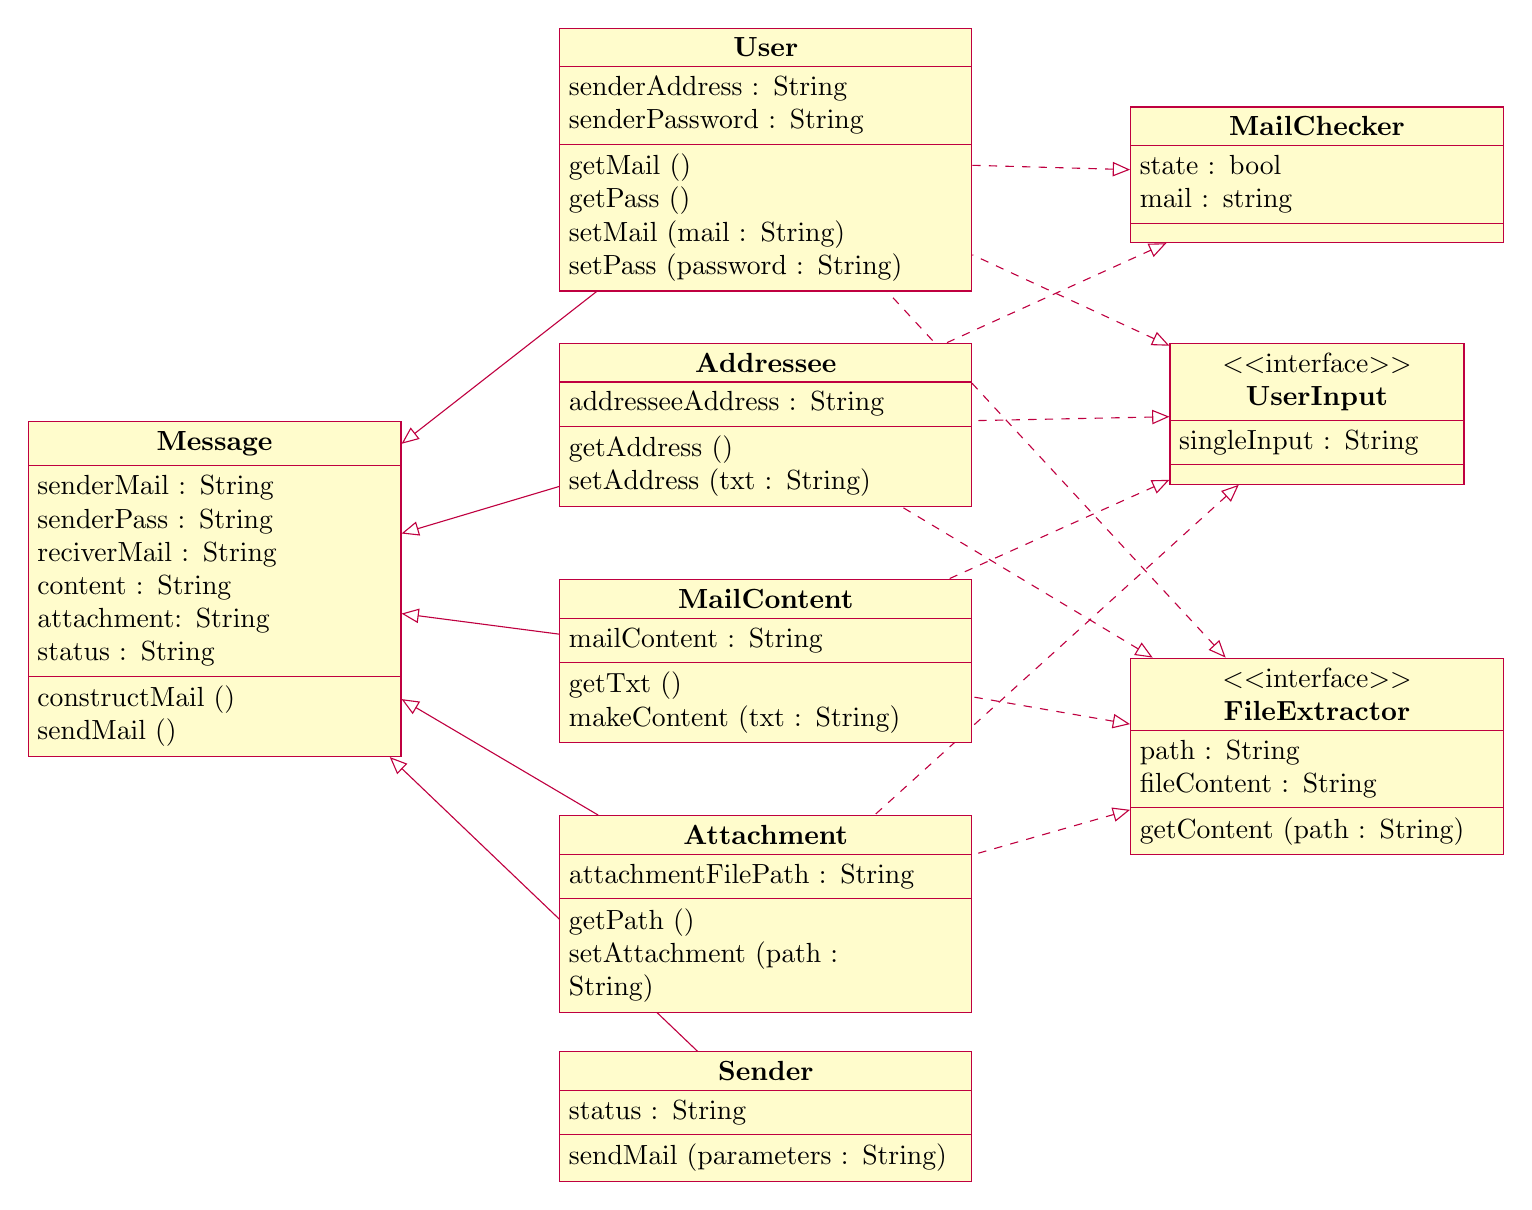
\begin{tikzpicture}
		\begin{class}[text width=4.5cm]{Message}{-5,-5}
			\attribute{senderMail : String}
			\attribute{senderPass : String}
			\attribute{reciverMail : String}
			\attribute{content : String}
			\attribute{attachment: String}
			\attribute{status : String}
			
			\operation{constructMail ()}
			\operation{sendMail ()}
		\end{class}
	
		\begin{interface}[text width=3.5cm]{UserInput}{9,-4}
			\attribute{singleInput : String}
		\end{interface}
	
		\begin{interface}[text width=4.5cm]{FileExtractor}{9,-8}
			\attribute{path : String}
			\attribute{fileContent : String}
			
			\operation{getContent (path : String)}
		\end{interface}
	
		\begin{class}[text width=4.5cm]{MailChecker}{9,-1}
			\attribute{state : bool}
			\attribute{mail : string}
		\end{class}
		
		\begin{class}[text width=5cm]{User}{2,0}
			\implement{UserInput}
			\implement{MailChecker}
			\implement{FileExtractor}
			\inherit{Message}
			\attribute{senderAddress : String}
			\attribute{senderPassword : String}
			
			\operation{getMail ()}
			\operation{getPass ()}
			\operation{setMail (mail : String)}
			\operation{setPass (password : String)}
		\end{class}
	
		\begin{class}[text width=5cm]{Addressee}{2,-4}
			\implement{UserInput}
			\implement{MailChecker}
			\implement{FileExtractor}
			\inherit{Message}
			\attribute{addresseeAddress : String}
			
			\operation{getAddress ()}
			\operation{setAddress (txt : String)}
		\end{class}
	
		\begin{class}[text width=5cm]{MailContent}{2,-7}
			\implement{UserInput}
			\implement{FileExtractor}
			\inherit{Message}
			\attribute{mailContent : String}
			
			\operation{getTxt ()}
			\operation{makeContent (txt : String)}
		\end{class}
		
		\begin{class}[text width=5cm]{Attachment}{2,-10}
			\implement{UserInput}
			\implement{FileExtractor}
			\inherit{Message}
			\attribute{attachmentFilePath : String}
			
			\operation{getPath ()}
			\operation{setAttachment (path : String)}
		\end{class}
		
		\begin{class}[text width=5cm]{Sender}{2,-13}
			\inherit{Message}
			\attribute{status : String}
			
			\operation{sendMail (parameters : String)}
		\end{class}

	\end{tikzpicture}
	
\end{document}